\documentclass{article}
\usepackage{amsmath}
\usepackage{tikz}

\begin{document}

\begin{figure}[h]
    \centering
    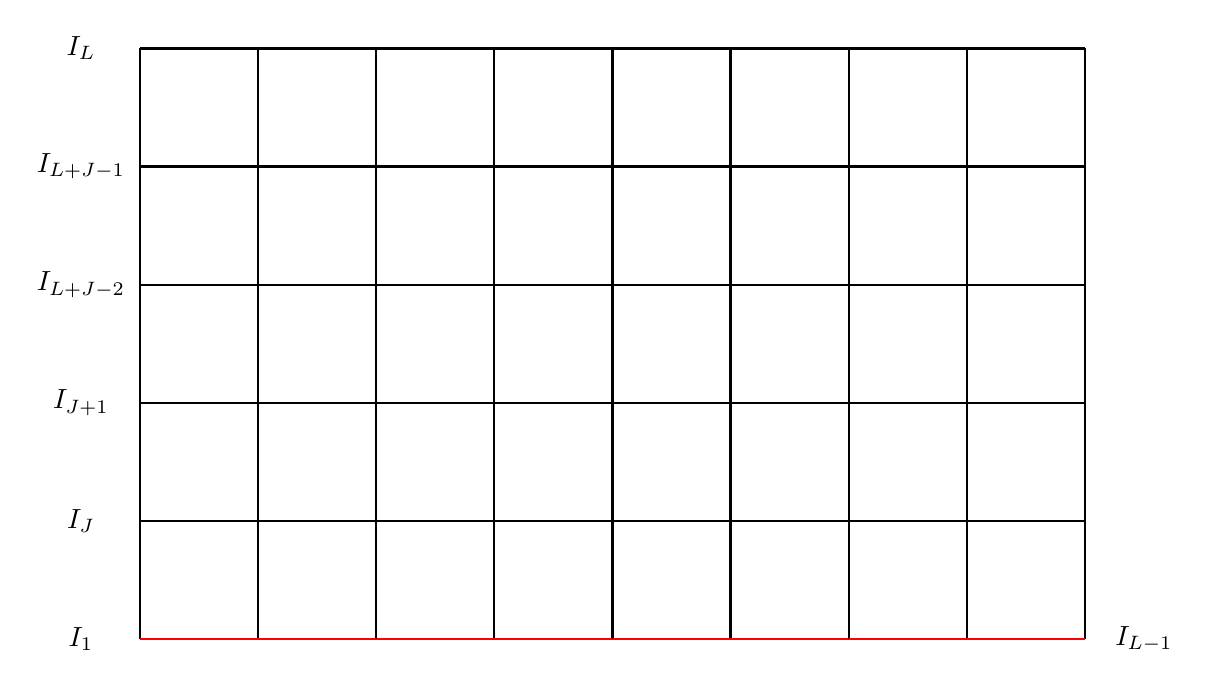
\begin{tikzpicture}[scale=1.5]
        % Draw horizontal lines for the intervals
        \draw[thick] (0,0) -- (8,0);
        \draw[thick] (0,1) -- (8,1);
        \draw[thick] (0,2) -- (8,2);
        \draw[thick] (0,3) -- (8,3);
        \draw[thick] (0,4) -- (8,4);
        \draw[thick] (0,5) -- (8,5);
        
        % Draw vertical lines for the intervals
        \draw[thick] (0,0) -- (0,5);
        \draw[thick] (1,0) -- (1,5);
        \draw[thick] (2,0) -- (2,5);
        \draw[thick] (3,0) -- (3,5);
        \draw[thick] (4,0) -- (4,5);
        \draw[thick] (5,0) -- (5,5);
        \draw[thick] (6,0) -- (6,5);
        \draw[thick] (7,0) -- (7,5);
        \draw[thick] (8,0) -- (8,5);
        
        % Label the intervals
        \node at (-0.5,0) {$I_1$};
        \node at (-0.5,1) {$I_J$};
        \node at (-0.5,2) {$I_{J+1}$};
        \node at (-0.5,3) {$I_{L+J-2}$};
        \node at (-0.5,4) {$I_{L+J-1}$};
        \node at (-0.5,5) {$I_L$};
        \node at (8.5,0) {$I_{L-1}$};
        
        % Dashed intervals
        \draw[dashed] (0,0) -- (8,0);
        \draw[dashed] (0,1) -- (8,1);
        \draw[dashed] (0,2) -- (8,2);
        \draw[dashed] (0,3) -- (8,3);
        \draw[dashed] (0,4) -- (8,4);
        \draw[dashed] (0,5) -- (8,5);
        
        % Red intervals
        \draw[red, thick] (0,0) -- (4,0);
        \draw[red, thick] (4,0) -- (8,0);
        
        % Dotted line between I_J and I_{L-1}
        \draw[dotted] (4,0) -- (4,5);
        \draw[dotted] (4,5) -- (8,5);
        
        % Dotted line between I_{L-2} and I_L
        \draw[dotted] (6,0) -- (6,5);
        \draw[dotted] (6,5) -- (8,5);
        
        % Dotted line between I_2 and I_{L-2}
        \draw[dotted] (2,0) -- (2,5);
        \draw[dotted] (2,5) -- (8,5);
        
        % Dotted line between I_2 and I_L
        \draw[dotted] (4,0) -- (4,5);
        \draw[dotted] (4,5) -- (8,5);
    \end{tikzpicture}
    \caption{This figure illustrates the instances created by Alice and Bob in the proof of Theorem~\ref{thm:lb-unit-length} for an instance of $\textsf{Index}_{L-2}$ with $X[J] = 1$. The dashed intervals on the upper part correspond to the zero elements of the bitvector $X$. The red intervals $I_1$, $I_2$ correspond to expired intervals. $I_J$ is the only non-expired interval disjoint with the special interval $I_{L-1}$. Since $X[J] = 1$, the optimal solution is of size $2$. If $X[J]$ was equal to $0$ then the interval $I_J$ would not be disjoint with $I_{L-1}$, and, thus, an optimal solution would be of size $1$.}
    \label{fig:lb-unit-length}
\end{figure}

\end{document}